\documentclass[11pt]{jreport}
\usepackage{geometry}
\usepackage{graduate}
\usepackage[dvipdfmx]{graphicx}
\usepackage{color}
\usepackage{amsmath,amssymb,amsthm,bm}
\usepackage{algorithm,algpseudocode}
\usepackage{float}
\usepackage{multicol}
\usepackage{caption}
\usepackage{verbatim}
\usepackage{calc}
\usepackage{enumitem}
\usepackage[
  style=ieee,backend=biber,
  texencoding=utf8,bibencoding=utf8,
  dashed=false,
  isbn=false,url=false,doi=false,eprint=false,
]{biblatex}
\renewbibmacro{in:}{}
\DeclareFieldFormat{journaltitle}{#1}
\DeclareFieldFormat{booktitle}{#1}
%\renewrobustcmd*{\bibinitdelim}{}
% theorem setting
\newtheoremstyle{mythmstyle}{}{}{\rmfamily}{}{\bfseries}{}{5pt}{}
\theoremstyle{mythmstyle}
\newtheorem{definition}{定義}
\newtheorem{lemma}{補題}
\newtheorem{theorem}{定理}
\newtheorem{corollary}{系}
\newtheorem{assumption}{仮定}
\newtheorem{example}{例}
%\newtheorem{algorithm}{アルゴリズム}
%
\renewcommand\proofname{\gt 証明\nopunct}
%\newenvironment{proof}{\par \noindent {\gt 証明}\ }{\hspace{\fill}$\Box$
%\vspace{0.5\baselineskip} \par}
%
% algorithm setting
\algnewcommand{\LeftComment}[1]{\(\triangleright\) #1}
\algrenewcommand\algorithmicindent{.5em}
\renewcommand{\listalgorithmname}{アルゴリズムリスト}
%\renewcommand{\thealgorithm}{\arabic{chapter}.\arabic{algorithm}}
\renewcommand{\thealgorithm}{\arabic{algorithm}}
\makeatletter
\renewcommand{\ALG@name}{アルゴリズム}
%\@addtoreset{algorithm}{chapter}
\makeatother
%
% path setting
\graphicspath{{../res/figure/}{./plot/}}
\makeatletter
\def\input@path{{../res/figure/}{./table/}}
\makeatother
\addbibresource{../res/MyCollection.bib}
%
% toc level setting
\setcounter{tocdepth}{1}
%
\title{○○に関する研究}
\author{Bubo bubo}
\date{平成28年2月5日} % 提出日
\reportname{修 士 論 文} 
\department{岡山大学大学院自然科学研究科電子情報システム工学専攻}
\supervisor{Ptilopsis leucotis}

\abst{
  媒介中心性はネットワークのノードの重要性をはかる指標として多く用いられている.
  媒介中心性を求めるアルゴリズムとしてBrandesのアルゴリズムが開発されて以来,多くのアルゴリズムが開発された.

  現実のネットワークは時間とともにリンクが出現したり消滅したりする時変ネットワーク
  であることから,そのようなネットワークの媒介中心性を効率的に計算する方法も開発されている.
  その中で,ネットワークの最短経路を保存する方法も提案されてきた.

  しかし,RamalingamとRepsの最短経路更新法に基づく辺削除時の媒介中心性更新アルゴリズムは知られていない.
  そこで,本研究ではRamalingamとRepsの最短経路更新アルゴリズムに基づく媒介中心性更新法を提案する.
  また,その方法の有効性を実験によって検証する.

  提案したアルゴリズムの最悪計算時間量はそのままであるが,
  末端の頂点に接続する辺の削除などの変化が少ない場合は
  効率的に最短経路および媒介中心性を更新できることが確認した.
  また,実験では,人工ネットワークと実ネットワークの両方でBrandesのアルゴリズムより高速に
  更新できることを確認した.しかし,辺が多く削除される場合はBrandesのアルゴリズムの方が
  高速に媒介中心性を計算することが確認された.
}


%
\begin{document}
\maketitle

\chapter{序論}

本章ではグラフの頂点の重要度を表す中心性と,更新アルゴリズムと,特に本研究と関連がある媒介中心性更新アルゴリズムについて述べる.

\section{中心性・媒介中心性}

中心性の提唱から各種中心性の特徴

媒介中心性を効率的に計算する方法の研究

\section{オンラインアルゴリズム}

一方,

\section{関連研究}

\section{メモ}

媒介中心性\cite{Freeman1977}はグラフの頂点の重要度を示す指標のひとつである.高い媒介中心性をもつ頂点は,多くの最短経路が通っていることを意味する.媒介中心性を求めるアルゴリズムとしてBrandesのアルゴリズム\cite{Brandes2001}が知られているが,辺の追加や削除といった操作がされると計算を最初から行う必要がある.

そこで,辺の操作に対して,各頂点の媒介中心性を高速に更新するアルゴリズムが開発されてきた.それらの中には,専用のデータ構造を用いるアルゴリズム\cite{Lee2012,Hayashi2015}や,最短経路長と最短経路数の更新を伴うアルゴリズム\cite{Pontecorvi2015,Bergamini2017}がある.また,PontecorviらはDemetrescuらの方法\cite{Demetrescu2003}を応用した方法を開発し\cite{Pontecorvi2015},BergaminiらはRamalingamらの方法\cite{Ramalingam1996}を応用して辺挿入に対する方法を開発した\cite{Bergamini2017}.

一方,Ramalingamらの方法に基づく辺削除時の媒介中心性更新アルゴリズムは知られていない.そこで,本稿ではRamalingamらの最短経路長更新アルゴリズムに基づく媒介中心性更新法を提案する.また,その方法の有効性を実験によって検証する.


%\chapter{ネットワーク科学}
\label{chap:network-science}

本章では,本研究に関連した分野であるネットワーク科学の概要と応用例について説明する.
その中でも,ネットワーク科学の応用例とネットワークノードの重要度を測る中心性について詳しく説明する.

\section{ネットワーク科学の成り立ち}

ネットワーク科学とは,二つの主体間の関係を表すデータの分析およびモデル化に関する研究分野である.
ここで言う主体とは,対象とする関係によって異なる.例えば,友人関係ならば,主体は個人を表し,食物連鎖の関係ならば,主体は動物の種を表す.
二つの主体間の関係を表すデータであれば主体の種類は問わない.
そのため,ネットワーク科学はあらゆる主体を対象にとることが可能という意味で普遍性を有する.
その考え方は,主にデータ構造の面で近いグラフ理論から引き継がれている.
その他,化学においては,分子同士の結合を記述するためにネットワーク構造が用いられたり\cite{Sylvester1878},
社会科学においては,人間関係をネットワーク構造として表したものをソシオグラムと呼んだり\cite{Moreno1978}
と複数の研究分野と相互に影響を与えている.

近年,高性能な計算機がが普及したことによって,現実にある膨大なネットワークを分析することが可能になった.
例えば,Twitterのフォローネットワーク\cite{Kwak2010}や,
StackExchangeでの回答ネットワーク\cite{Movshovitz-Attias2013},
GitHubのコラボレーションネットワーク\cite{Lima2014}が挙げられる.
これらの分析により,人のミクロな交流をマクロな視点で考察できるようになった.

その一方,現実のネットワークの特徴を上手く表現するようなモデルが開発されてきた.
古くからあるモデルは1959年にErd{\"{o}}sとR{\'{e}}nyiが開発したランダムグラフ\cite{Erdos1959}で,
完全グラフからランダムに辺を取り出す操作を繰り返すことで得られる.
近年では,ネットワークに見られる六次の隔たり\cite{Travers1969}の特徴を表した
WattsとStrogatzのスモールワールドネットワーク\cite{Watts1998}や,
次数分布がべき分布であるスケールフリー性を再現した,Barab{\'{a}}siとAlbertによる
スケールフリーネットワーク\cite{Barabasi1999}が開発された.
それに加えて,既存のネットワークに新たな概念を加えたネットワークモデルも考案されている.
主なモデルは,主体の関係が時々刻々と変化するテンポラルネットワーク(時変ネットワーク)\cite{Holme2012}や,
職場とサークルなど,同じ主体の組み合わせで関係が複数あるものの議論を可能にする多層ネットワーク\cite{Kivela2014}がある.

\section{ネットワーク科学の応用例}

以後,ネットワーク科学のいくつかの応用を示す.まず,ネットワーク科学の応用として注目され続ける
感染症の伝搬について説明する.その後,本研究の応用として考えられる交通網と社会ネットワークの分析
について説明する.
本章で説明していないネットワーク科学と社会との関係や,
その他の応用は,Barab{\'{a}}siの著書\cite{Barabasi2016}に詳しく記されている.

\subsection{感染症の伝搬}

インフルエンザやエボラ出血熱など,感染症の中には我々の脅威となるものがある.
古くは14世紀にヨーロッパで流行したペスト,18世紀から19世紀にかけて世界的に流行したコレラ,
20世紀初頭に流行したスペイン風邪がある.
そのような感染症の対策として,その病理の解明と同時に感染の規模を予測することも重要である.

20世紀以前の感染症拡散のモデルはひとつの空間に基づくもので,これは同じ社会物理的な空間にいるならば,
感染する可能性があるとするものだった.つまり,駅構内や病院などの一定の広さの空間のみを対象としていた.

その一方,Hufnagelらのモデル\cite{Hufnagel2004}は,従来の局所的な感染に加え,
感染者が飛行機で移動し,その感染者から感染することも考慮されている.
この感染症予測は,インフルエンザあるいはエボラ出血熱の流行の予測に用いられる.
実際,そのモデルは2009年に発生したH1N1型インフルエンザウイルスによるパンデミックの
規模を正確に予測した\cite{Balcan2009}.

また,この手法を用いると,生物を媒介とするウイルスの他に,コンピュータウイルスや社会的なウイルスの
ミームの拡散を予測することも可能である.
例えば,Wangらは2010年に携帯電話を媒介するコンピュータウイルスが拡散する条件を予測した\cite{Wang2009}.

\subsection{交通網の分析}

感染症の予測では空の交通網が活用されていたが,陸の交通網である道路もネットワーク科学で分析できる.
特に,頑健な社会インフラの構築のために,交通網の脆弱な箇所を見つけて保全することは重要である.

2007年にTaylorらは,高速道路をネットワークとみなすことで,交通網の脆弱な箇所を特定した\cite{Taylor2007}.
Taylorらによる道路ネットワークの頑健性の概念には,信頼性と脆弱性がある.
信頼性とはある時間の水準で車が到達できるかを表す.道路の通行のしやすさおよび移動できる確率に依存する.
一方,脆弱性とは道路が不全になった時に引き起こされる社会的,経済的な影響の大きさを表す.
Taylorらは,これらの概念に対する簡単な指標を定義して,実際のオーストラリアの主要道路を分析した.

2010年,Tizghadamらは,交通網のネットワークの頑健性を最適化するために,
道路の許容量を調整する進化計算のアルゴリズムを開発した\cite{Tizghadam2010}.
Tizghadamらのネットワークの頑健性は後に説明する媒介中心性の派生に基づいている.
その指標はランダムウォークの考え方に基づき,その指標が高い地点はより頻繁に通過される地点であることを表す.

\subsection{社会ネットワークの分析}

社会ネットワークとは,もともとは学校や職場といった特定の集団に属するネットワークを指す.
この考え方を使って,学校や職場など,特定の集団の中にある個人の心理学について議論された\cite{Moreno1978}.
しかし,近年では,ソーシャルネットワーキングサービスの台頭により,従来とは比較にならない程大きなネットワークが取得可能となった.
それにより,特定の集団に限定されない,より巨視的な議論が可能となった.

その一つに,巨大なネットワークを特定の集団に分けるコミュニティ検出\cite{Fortunato2010}が挙げられる.
古典的には,最小カット問題を解く要領でネットワークを分割する方法や,
類似するノードを同じコミュニティにまとめることを繰り返す方法がある.
後者は事前にコミュニティの数を与える必要がないことが利点である.
また,隣接行列をふたつの行列の積を用いて近似することを応用した方法\cite{Wang2011}もある.

また,オンラインゲームの利用者同士の協力行動の理解も試みられている.
Szellらは,多層ネットワークの考え方を使って,オンラインゲームの利用者間の交流を分析した\cite{Szell2010}.
その結果,攻撃などの負の関係で構築されたネットワークはべき次数分布を示すことが分かった.
特に,敵対関係のネットワークは優先的選択\cite{Barabasi1999}で構築される.
さらに,友好などの正の関係のネットワークのクラスタリング係数は,負の関係のネットワークのものより高いことも分かった.
クラスタリング係数が高いネットワークは,その凝集性から協力関係が広がりやすいことが知られている.

ネットワークを分析するに当たって,ネットワーク内の重要なノードを発見することは有意義である.
次節では,重要なノードの発見や,ノードの重要性の計測に役立つ中心性について述べる.

\section{中心性}
\label{sect:centrality}

組織内の重要な人物を発見することは古くからの組織論の課題である\cite{Christie1952,Ibarra1993}.
ネットワークのノードの重要度は中心性と呼ばれ,用途に沿っていくつかの中心性が開発されてきた.
その中で最も単純なものは各ノードの次数(隣接しているノードの数)をそのまま使う次数中心性である.
しかし,次数が高くても真に重要であるとは限らない.
例えば,フォロワー数が数万だとしても,そのほとんどが機械的に
運用されているアカウントであれば,真に影響力を持っているとは言い難い.
この節では以下,現在まで提案された主な中心性について説明する.
グラフ理論の記号および意味に関しては,第\ref{chap:preliminary}章を参照されたい.

\subsection{近接中心性}
\label{subsect:closeness}

近接中心性\cite{Bavelas1948,Beauchamp1965}とは,
ネットワーク内の他のノードとの距離の総和の逆数として定義される.つまり,
\begin{equation*}
  C_v=\cfrac{1}{\sum_wd_{v,w}}.
\end{equation*}

近接中心性が高いノードは他のノードに近い位置にあり,ここから情報を伝達すると
情報を速く伝達できると考えられる.
しかし,この定義の通信モデルは最短経路を通ることを仮定しているので,
別の通信モデルでは現実的でないことがある.
これを考慮して,ランダムウォークに基づく近接中心性も提案されている\cite{White2003}.

\subsection{媒介中心性}
\label{subsect:betweenness}

媒介中心性\cite{Anthonisse1971,Freeman1977}とは,
頂点ペア$(s,t)$の最短経路数に占める,自身を通る最短経路数の割合の総和として
定義される.つまり,
\begin{equation*}
  B_v=\sum_{s\neq v}\sum_{t\neq {v,s}}\frac{\sigma_{st}(v)}{\sigma_{st}}.
\end{equation*}

媒介中心性の大きなノードは多くの最短経路上にあり,通信に欠かせないノードであると言える.
近接中心性と同じく,この定義の通信モデルは最短経路を通ることを仮定しているので,
別の通信モデルでは現実的でないことがある.
これを考慮して,ランダムウォークに基づく媒介中心性も提案されている\cite{Newman2005}.

\subsection{固有ベクトル中心性}
\label{subsect:eigenvector}

固有ベクトル中心性(Eigenvector centrality)\cite{Bonacich1991}とは,
隣接する頂点の固有ベクトル中心性の総和として表現される.
つまり,$\lambda$を定数として,
\begin{equation*}
  x_v=\frac{1}{\lambda}\sum_{w\in\mathcal{N}_G(v)}x_w.
\end{equation*}
また,$\mathbf{A}$をグラフの隣接行列とすると,固有ベクトル方程式として表すことができる.
\begin{equation*}
  \mathbf{A}\mathbf{x}=\lambda\mathbf{x}.
\end{equation*}
一般に$\mathbf{A}$の固有値は複数存在するが,$\lambda$は$\mathbf{A}$の最大の固有値とする.

固有ベクトル中心性は,隣接する頂点の固有ベクトル中心性が高いほど自身の中心性も高いので,
Webページや学術論文誌のスコアリングに応用される.

%
\chapter{関連研究}
\label{chap:related-work}

本章では関連研究を説明する.また,本研究で提案するアルゴリズムの特徴を説明し,研究目的を述べる.

Freemanによる媒介中心性の定義を,定義通りそのまま求めるとき,その時間計算量は$\mathcal{O}(|V|^3)$である.
Brandesのアルゴリズム\cite{Brandes2001}は,ペア依存度を積算することにより媒介中心性を効率的に計算する.その時間計算量は$\mathcal{O}(|V||E|+|V|^2\log|V|)$である.
この考え方は,この後に提案されるアルゴリズムのほぼすべてに採用されている.以下,媒介中心性を求める手法を,
対象とする問題や特徴に分け,それぞれのグループに属する手法について簡単に説明する.

\section{静的グラフ}
本研究で取り扱う動的グラフでのアルゴリズムを説明する前に,操作が行われないようなグラフの媒介中心性計算アルゴリズムを説明する.
YangとChen\cite{Yang2011}は重み付きグラフの辺を分割するように頂点を挿入し,重みなしグラフとして計算することによって,
重み付きグラフの時間計算量を小さくする手法を提案した.
Puzisら\cite{Puzis2012}は二種類の前処理(構造的に等しい頂点を同一視するものと,クリークに基づき,グラフを木としてみなすもの)
によって,高速化する手法を提案した.
GreenとBader\cite{Green2013}は,ペア依存度の積算に必要な情報を,最短経路の探索時に保存するのではなく,
ペア依存度の積算時にオンデマンドで計算することによって空間計算量を削減する手法を提案した.
Erd{\"{o}}sら\cite{Erdos2015}は,分割統治法に基づいて,Brandesのアルゴリズムを書き換えた.
つまり,グラフを互いに素な部分グラフに分割し,それらの媒介中心性を求め,その後,それらを合わせる方法である.
Bentertら\cite{Bentert2018}は,前処理により次数が1または2の頂点を取り除きグラフを簡単にすることで,
実ネットワークのトポロジの媒介中心性を効率的に計算する方法を提案した.

\subsection{並列アルゴリズム}
一方,GPGPUなどハードウェアが普及したことにより,並列計算により媒介中心性を求める方法も提案されてきた.
BaderとMadduri\cite{Bader2006}は,最短経路の計算およびペア依存度の積算を粗粒に並列化することで,高速化を図った.
Tanら\cite{Tan2009}は,並列ランダムアクセス機械(並列的読み取り/排他的書き込み)上で,
最短経路の計算およびペア依存度の積算の処理を細粒に並列化することで媒介中心性の計算を高速化させた.
Edmondsら\cite{Edmonds2010}は,最短経路を計算する方法として$\Delta$--ステップ法を採用することで,
並列的読み取り/並列的書き込みの機械上でメモリ使用量を抑えた計算法を提案した.
ShiとZhang\cite{Shi2011}は,同じく$\Delta$--ステップ法を採用し,GPGPU上に媒介中心性を計算するプログラムを実装した.
Sariy{\"{u}}ceら\cite{Sariyuce2013}は,同じく$\Delta$--ステップ法を,辺について並列化させGPGPU上に実装した.
Bernaschiら\cite{Bernaschi2016}は,同行,同列でデータを共有できる2次元構造のプロセッサを駆使し,
最短経路の計算とペア依存度の積算を並列に実行する方法を提案した.

\subsection{近似アルゴリズム}
ネットワークが大きくなるにつれ,通常のBrandesのアルゴリズムでも計算に時間がかかる場合が多くなった.
そこで,媒介中心性の近似値を求めるアルゴリズムが提案されてきた.
主に二つのアプローチがあり,一つは全頂点間の最短経路を求めるのではなく,ピボットと呼ばれる部分頂点集合の頂点に限定して
最短経路の計算とペア依存度の積算を行い,ペア依存度を外挿することで媒介中心性を求める方法である\cite{Brandes2007}.
BrandesとPich\cite{Brandes2007}やBader\cite{Bader2007}によってこの方法が提案されてから,
より良いピボットの選択方法\cite{Geisberger2008,Chehreghani2014}や,
標本の表現力を表すVapnik-Chernovenkis次元に基づくピボット選択数の改良\cite{Riondato2014}や,
同じく標本の表現力を表すRademacher複雑度に基づくピボット選択数の改良\cite{Riondato2016}が提案された.

他にも,PfefferとCarleyによる,最短距離に上限を設ける方法\cite{Pfeffer2012}や,
Yoshidaによる,媒介中心性を符号化する働きをもつHypergraph Sketchを利用する方法\cite{Yoshida2014},
BorassiとNataleによる,ランダムに選択した二頂点間の最短経路を双方向幅優先探索により求め,
それを繰り返す方法\cite{Borassi2019}がある.

\section{動的グラフ}
第\ref{chap:network-science}章で説明した通り,現実のネットワークは時間によってその接続が変化することが多い.
そのため,グラフに何かしらの変更がされたときに媒介中心性の値を更新するアルゴリズムが求められる.
この問題を解くための知られているもっとも古いアルゴリズムはLeeら\cite{Lee2012}で,
Minimum union cycleと呼ばれる閉路の集合と媒介中心性を保持し,辺が変更されたときに媒介中心性を更新する方法である.
また,Singh\cite{Singh2015}は,この方法を応用し,頂点に変更があったときの媒介中心性を更新する方法を提案した.

その一方,最短経路やそれに関する値を保存する方法も提案されている.
Greenら\cite{Green2012}は,辺が挿入されたときの最短距離と最短経路の数と共に媒介中心性を更新する方法を提案し,
Nasreらが\cite{Karger1993}の方法を動的グラフに応用して,辺挿入時の媒介中心性を更新する方法を開発した\cite{Nasre2014a}.
また,Kasら\cite{Kas2013}は,RamalingamとRepsの最短経路更新法\cite{Ramalingam1996}を応用して,
辺挿入時の媒介中心性を更新する方法を開発した.
また,Nasreら\cite{Nasre2014b}は,DemetrescuとItalianoの最短経路更新法\cite{Demetrescu2003}を,複数の経路に一般化して,
辺削除時の媒介中心性を更新する方法を開発した.
さらに,PontecorviとRamachandran\cite{Pontecorvi2015}は,DemetrescuとItalianoの最短経路更新法を応用して
頂点追加時の媒介中心性をより効率的に更新する方法を開発した.
Kourtellisらは,重みなしグラフの頂点媒介中心性と辺媒介中心性の両方を更新する方法を開発した\cite{Kourtellis2015}.
Bergaminiらは,RamalingamとRepsのアルゴリズムを基に,辺挿入時の媒介中心性更新アルゴリズムを開発した\cite{Bergamini2017}.
このアルゴリズムは,ペア依存度を陽に保存せず,媒介中心性の値を直接更新することでメモリ使用量を削減している.
Jamourらは,articulation pointと媒介中心性の変化量の性質を示して,辺更新時の媒介中心性を更新するアルゴリズムを開発した\cite{Jamour2017}.
媒介中心性と最短経路を同時に更新するアルゴリズムを表\ref{tab:comparizon-of-algorithms}に示す.

なお,更新問題を解くにあたり,近似アルゴリズムや並列計算が用いられることがある.
例えば,Hayashiらは,\cite{Yoshida2014}のHypergraph sketchに加えて,Two-ball indexとSpecial-purpose reachability indexを追加することで,
グラフが操作された後の媒介中心性の近似値を計算する手法を開発した\cite{Hayashi2015}.
また,Bergaminiらは,\cite{Riondato2014}をグラフが変更されたときの媒介中心性の近似値を求めるアルゴリズムに応用した\cite{Bergamini2015a,Bergamini2015b}.
また,ChernoskutovらはGraph coarsingと呼ばれる媒介中心性が大きい頂点を残す前処理によって,辺挿入時の媒介中心性の近似値を求めるアルゴリズムを開発した\cite{Chernoskutov2015}.
さらに,Jamourらの方法\cite{Jamour2017}はその多くの部分が並列計算可能である.

\section{研究目的}
現在まで多くの媒介中心性更新アルゴリズムが提案されてきた一方,
Ramalingamらの方法に基づく辺削除時の媒介中心性更新アルゴリズムは知られていない.そこで,本稿ではRamalingamらの最短経路長更新アルゴリズムに基づく媒介中心性更新法を提案する.また,その方法の有効性を実験によって検証する.

\begin{table}[tb]
  \label{tab:comparizon-of-algorithms}
  \centering
  \caption{最短経路と共に媒介中心性を更新するアルゴリズム}
  \begin{tabular}{ccc}
    \hline
    アルゴリズム & 最短経路更新アルゴリズム & 辺の操作 \\ \hline
    Kasら\cite{Kas2013} & Ramalingamら\cite{Ramalingam1996} & 挿入 \\ \hline
    Nasreら\cite{Nasre2014a} & Kargerら\cite{Karger1993} & 挿入 \\ \hline
    Nasreら\cite{Nasre2014b} & Demetrescuら\cite{Demetrescu2003} & 削除 \\ \hline
    Pontecorviら\cite{Pontecorvi2015} & Demetrescuら\cite{Demetrescu2003} & 挿入/削除 \\ \hline
    Bergaminiら\cite{Bergamini2017} & Ramalingamら\cite{Ramalingam1996} & 挿入 \\ \hline
    本研究 & Ramalingamら\cite{Ramalingam1996} & 削除 \\ \hline
  \end{tabular}
\end{table}

\chapter{準備}

\section{グラフの数学的記法}
\label{sect:graph-theory}

グラフ$G=(V,E)$,$V$は頂点集合,$E$は辺集合$\subset V\times V$

辺集合が非順序対の集合であるとき,グラフは無向と呼ばれる.
逆に,辺集合が順序対の集合であるとき,グラフは有向と呼ばれる.

また,無向グラフの各辺$\{v,w\}\in E$および有向グラフの各辺$(v,w)\in E$には正の重み$l_{vw}>0$を与えている.

隣接する,接続している
$G$の頂点$v$の近傍$\mathcal{N}_G(v)$

頂点とそれに接続している辺が交互に並び,両端が頂点である列を有向道と呼ぶ.
記号と用いると,
\[ (v_1,e_1,v_2,\ldots,v_{n-1},e_n,v_n)\ (v_i\in V,\ e_i\in E) \]
である.
有向道は有向グラフとみなすことができ,例えば,有向道
\[ (v_1,e_1,v_2,\ldots,v_{n-1},e_{n-1},v_n) \]
を有向グラフとして表すと$G=(V,E)=(\{v_1,\ldots,v_n\},\{e_1,\ldots,e_{n-1}\})$である.

$G$の異なる2頂点$s,t$を両端とする有向道の中で,有向道に含まれる辺の重みの総和が最小であるものを,$s$から$t$への最短経路と呼ぶ.
頂点$s$から頂点$t$への最短経路の辺の重みの総和を最短経路長$d_{st}$,最短経路の数を最短経路数$\sigma_{st}$と呼ぶ.
以下の議論では,便宜上,すべての$s\in V$に対し$d_{ss}=0$, $\sigma_{ss}=1$とする.
また,$s$から$t$への最短経路の中で頂点$v$を通るものの個数を$\sigma_{st}(v)$で表す.
頂点$s$から他の頂点へのすべての最短経路で構成される有向グラフを$G_s=(V_s,E_s)$で表す.
同様に,頂点$s$から頂点$t$へのすべての最短経路で構成される有向グラフを$G_{st}=(V_{st},E_{st})$で表す.

\section{最短経路長および最短経路数の性質}
\label{sect:shortest-paths}

最短経路の長さと個数について,いくつかの補題を示す.

\begin{lemma}[Brandes~\cite{Brandes2001}]
  $G=(V,E)$の異なる2頂点$s,t \in V$に対して,$s$から$t$への最短経路$G_{st}=(V_{st},E_{st})$が$i \in V$を含む,すなわち$i \in V_{st}$であるための必要十分条件は
  \begin{equation}
    d_{st}=d_{si}+d_{it}
    \label{eqn:inclusion0}
  \end{equation}
  が成り立つことである.
  \label{lemma:1}
\end{lemma}
\begin{proof}
  はじめに$i=s$の場合を考える.このとき明らかに$i \in V_{st}$であり,かつ$d_{si}+d_{it}=d_{ss}+d_{st}=d_{st}$より\eqref{eqn:inclusion0}もつねに成り立つ.$i=t$の場合も同様である.そこで以下では$i \not\in \{s,t\}$と仮定する.$G_{st}$が頂点$i$を含むならば,$G_{st}$の中に$s \rightarrow \cdots \rightarrow i \rightarrow \cdots \rightarrow t$の順に頂点を通る有向道が存在する.この有向道の長さは$d_{si}+d_{it}$で与えられるので\eqref{eqn:inclusion0}が成り立つ.次に\eqref{eqn:inclusion0}が成り立つと仮定する.頂点$s$を出発して$s$から$i$への最短経路の一つを通って$i$に行き,次に$i$から$t$への最短経路の一つを通って$t$に行く有向道を考える.この有向道は$s$から$t$への最短経路の一つである.なぜなら,その長さは$d_{si}+d_{it}$で与えられ,\eqref{eqn:inclusion0}より$s$から$t$への最短経路長$d_{st}$に等しいからである.したがって$i \in V_{st}$が成り立つ.
\end{proof}

\begin{lemma}
  $G=(V,E)$の異なる2頂点$s,t\in V$と辺$\{i,j\} \in E$を考える.$s$から$t$への最短経路$G_{st}=(V_{st},E_{st})$が有向辺$(i,j)$を含む,すなわち$(i,j) \in E_{st}$が成り立つための必要十分条件は
  \begin{equation}
    d_{st}=d_{si}+l_{ij}+d_{jt}
    \label{eqn:inclusion}
  \end{equation}
  が成り立つことである.
  \label{lemma:2}
\end{lemma}
\begin{proof}
  はじめに$i=s$, $j=t$の場合を考える.このとき明らかに$G_{st}$は
  有向辺$(i,j)$を含み,かつ$d_{si}+l_{ij}+d_{jt}=d_{ss}+l_{st}+d_{tt}=l_{st}=d_{st}$
  より\eqref{eqn:inclusion}も成り立つ.次に$i=s$, $j \neq t$の場合を
  考える.このとき$(i,j)\in E_{st}$であるための必要十分条件は$G_{st}$が
  $j$を含むことである.これは補題~\ref{lemma:1}より
  $d_{st}=d_{sj}+d_{jt}$と等価であり,さらに右辺$d_{sj}+d_{jt}$は
  \eqref{eqn:inclusion}の右辺と等しい.$i\neq s$, $j=t$の場合も同様である.
  そこで以下では$s,t,i,j$がすべて異なると仮定する.
  $G_{st}$が有向辺$(i,j)$を含むならば,$G_{st}$の中に
  $s \rightarrow \cdots \rightarrow i \rightarrow j \rightarrow \cdots \rightarrow t$
  の順に頂点を通る有向道が存在する.
  この有向道の長さは$d_{si}+l_{ij}+d_{jt}$で与えられるので\eqref{eqn:inclusion}が
  成り立つ.次に\eqref{eqn:inclusion}が成り立つと仮定する.頂点
  $s$を出発して$s$から$i$への最短経路の一つを通って$i$に行き,次に
  辺$\{i,j\}$を通って$j$に行き,最後に$j$から$t$への最短経路の一つを
  通って$t$に行く有向道が存在する.この有向道は$s$から$t$への最短経路の一つで
  ある.なぜなら,その長さは$d_{si}+l_{ij}+d_{jt}$で与えられ,
  \eqref{eqn:inclusion}より$s$から$t$への最短経路長$d_{st}$に
  等しいからである.したがって,$(i,j) \in E_{st}$が成り立つ.
\end{proof}

\begin{lemma}[Brandes\cite{Brandes2001}]
  $G=(V,E)$の異なる2頂点$s,t \in V$に対して,
  $s$から$t$への最短経路の中で$i$を通るものの個数$\sigma_{st}(i)$は
  次式で与えられる.
  \begin{equation}
    \sigma_{st}(i)=
    \left\{
    \begin{array}{ll}
      \sigma_{si} \sigma_{it}, & d_{st}=d_{si}+d_{it}\,\mbox{のとき} \\
      0, & \mbox{それ以外のとき}
    \end{array}
    \right.
    \label{eqn:sigma_sti}
  \end{equation}
  \label{lemma:3}
\end{lemma}

\begin{lemma}
  $G=(V,E)$の異なる2頂点$s,t \in V$に対して,
  $s$から$t$への最短経路の中で有向辺$(i,j)$を通るものの個数を
  $\sigma_{st}(i,j)$とおくと,それは次式で与えられる.
  \begin{equation*}
    \sigma_{st}(i,j)=
    \left\{
    \begin{array}{ll}
      \sigma_{si} \sigma_{jt}, & d_{st}=d_{si}+l_{ij}+d_{jt}\,\mbox{のとき} \\
      0, & \mbox{それ以外のとき}
    \end{array}
    \right.
    %\label{eqn:sigma_stij}
  \end{equation*}
  \label{lemma:4}
\end{lemma}

次の補題は,ある二頂点間の最短経路の長さと,その経路に含まれる短い最短経路の長さに関するものである.
\begin{lemma}
  \label{lemma:distance-of-path}
  $G=(V,E)$の異なる二頂点$s,t\in V$について,次が成り立つ.
  \begin{equation*}
    d_{st}=\min\{d_{si}+d_{it}|i\in V\}
  \end{equation*}
\end{lemma}
\begin{proof}
  \textcolor{red}{TODO}
\end{proof}

次の補題は,重みなしグラフのある二頂点間の最短経路の個数と,その経路に含まれる短い最短経路の個数との関係を示す.
\begin{lemma}
  \label{lemma:number-of-paths}
  重みなしグラフ$G=(V,E)$の異なる二頂点$s,t\in V$について,$v$を$d_{st}=d_{sv}+d_{vt}$
  である頂点(ただし$v\neq s,t$)とすると,次が成り立つ.
  \begin{equation}
    \label{eq:number-of-paths}
    \sigma_{st}=\frac{\sum_{v}\sigma_{sv}\sigma_{vt}}{d_{st}-1}
  \end{equation}
\end{lemma}
\begin{proof}
  $s$と$t$の間の一般的な経路を図\ref{fig:proof-number-of-paths}に示す.
  \begin{figure}
    \centering
    \def\svgwidth{.5\columnwidth}
    \input{proof-number-of-paths.pdf_tex}
    \caption{$s$と$t$の一般的な最短経路}
    \label{fig:proof-number-of-paths}
  \end{figure}
  $s$からの距離が一定の頂点を並べて,一つの層とする.$d_{sv}=k$なる頂点$v$の集合を,第$k$層と定義し,$L_k$と表す.$L_k$に属する頂点の数を$n_k$,$L_k$に属する$l$番目の頂点を$v_{kl}$と表す.ここで,第$k$層に属する頂点$v$は,隣接する層(第$k-1$層と第$k+1$層)以外の層に属する頂点$w$と隣接しないことに注意する.もしそのような頂点が存在すると,最短経路長が変化する.式\eqref{eq:number-of-paths}の両辺に$d_{st}-1$を掛けて,次の式\eqref{eq:number-of-paths1}を得る.
  \begin{equation}
    \sigma_{st}(d_{st}-1)=\sum_{v}\sigma_{sv}\sigma_{vt}
    \label{eq:number-of-paths1}
  \end{equation}
  式\eqref{eq:number-of-paths1}の右辺を,
  図\ref{fig:proof-number-of-paths}にならって表すと,
  \begin{equation}
    \sum_{v}\sigma_{sv}\sigma_{vt}=
    \sum_{k=1}^m\sum_{l=1}^{n_k}\sigma_{sv_{kl}}\sigma_{v_{kl}t}
    \label{eq:number-of-paths2}
  \end{equation}
  が得られる.ここで,二つの頂点$v$と$w$について,次の隣接を表す記号$a$を導入する.
  \begin{align*}
    a_{vw}=
    \begin{cases}
      1 & vとwが隣接しているとき \\
      0 & vとwが隣接していないとき
    \end{cases}
  \end{align*}
  各々の$\sigma_{sv_{kl}}\sigma_{v_{kl}t}$について議論する.$a$の定義を用いて式を変形すると,
  \begin{align}
    &\sigma_{sv_{kl}}\sigma_{v_{kl}t}\nonumber\\
    =&\left(\sum_{v'\in L_{k-1}}\sigma_{sv'}a_{v'v_{kl}}\right)
    \left(\sum_{v'\in L_{k+1}}\sigma_{v_{kl}v'}a_{v't}\right)
    \nonumber\\
    =&\left(\sum_{v''\in L_{k-2}}\sum_{v'\in L_{k-1}}
    \sigma_{sv''}a_{v''v'}a_{v'v_{kl}}\right)
    \left(\sum_{v'\in L_{k+1}}\sum_{v''\in L_{k+2}}
    a_{v_{kl}v'}a_{v'v''}\sigma_{v''t}\right)
    \nonumber\\
    &\vdots\nonumber\\
    =&\left(\sum_{(v_1,\ldots,v_{k-1})\in L_1\times\cdots\times L_{k-1}}
    a_{sv_1}\cdots a_{v_{k-1}v_{kl}}\right)
    \left(\sum_{(v_{k+1},\ldots,v_m)\in L_{k+1}\times\cdots\times L_m}
    a_{v_{kl}v_{k+1}}\cdots a_{v_mv_t}\right)\nonumber\\
    =&\sum_{(v_1,\ldots,v_{k-1},v_{k+1},\ldots,v_m)\in L_1\times\cdots\times L_{k-1}\times L_{k+1}\times\cdots\times L_m}
    a_{sv_1}\cdots a_{v_{k-1}v_{kl}}a_{v_{kl}v_{k+1}}\cdots a_{v_mt}
    \label{eq:number-of-paths3}
  \end{align}
  が得られる.式\eqref{eq:number-of-paths3}を式\eqref{eq:number-of-paths2}に
  代入すると,
  \begin{align}
    &\sum_{k=1}^m\sum_{l=1}^{n_k}\sigma_{sv_{kl}}\sigma_{v_{kl}t}\nonumber\\
    =&\sum_{k=1}^m\sum_{l=1}^{n_k}\sum_{
      (v_1,\ldots,v_{k-1},v_{k+1},\ldots,v_m)\in
      L_1\times\cdots\times L_{k-1}\times L_{k+1}\times\cdots\times L_m
    }a_{sv_1}\cdots a_{v_{k-1}v_{kl}}a_{v_{kl}v_{k+1}}\cdots a_{v_mt}\nonumber\\
    =&\sum_{k=1}^m\sum_{(v_1,\ldots,v_m)\in L_1\times\cdots\times L_m}
    a_{sv_1}\cdots a_{v_mt}\nonumber\\
    =&m\left(\sum_{(v_1,\ldots,v_m)\in L_1\times\cdots\times L_m}
    a_{sv_1}\cdots a_{v_mt}\right)
    \label{eq:number-of-paths4}
  \end{align}
  と変形できる.式\eqref{eq:number-of-paths4}の総和の対象が$1$となるのは,
  $a_{sv_1},\ldots,a_{v_mt}$のすべてが$1$のとき,
  すなわち,$s$と$v_1$,$v_1$と$v_2$,$\ldots$,$v_m$と$t$がすべて隣接している
  とき,すなわち,$s$と$t$の最短経路となっているときである.
  従って,総和の値は$s$と$t$の最短経路の数と一致し,
  式\eqref{eq:number-of-paths4}は$\sigma_{st}(d_{st}-1)$と等しい.
  従って,補題が成り立つ.
\end{proof}

\section{媒介中心性とペア依存度}
\label{sect:pairwise-dependency}

頂点$i$の媒介中心性$B_i$は
\begin{equation}
  B_i=\sum_{s\neq i}\sum_{t\neq {i,s}}\frac{\sigma_{st}(i)}{\sigma_{st}}
  \label{eq:betweenness-centrality}
\end{equation}
で定義される\cite{Freeman1977}.
すなわち,頂点$i$の媒介中心性は$s$から$t$への最短経路の個数とその中で頂点$i$を通るものの個数の比を$s,t$のすべての組について足し合わせたものである.したがって,媒介中心性の大きな頂点は多くの2頂点を結ぶ最短経路上にあり,この意味で重要度が高いと言える.

すべての頂点の媒介中心性を求める単純な方法は以下の通りである.まず,$s=1,2,\ldots,N$に対して,幅優先探索を用いて$s$から他のすべての頂点への最短経路を求める.その過程で,$s$から他のすべての頂点への最短経路長と最短経路数も同時に求める.次に,互いに異なる3頂点の組$\{s,t,i\}$のすべてに対して,$\sigma_{st}(i)$の値を計算する.
最後に媒介中心性$B_i$ $(i=1,2,\ldots,N)$を(\ref{eq:betweenness-centrality})により計算する.しかしながら,この方法の計算量は$\mathcal{O}(N^3)$であり,大規模なネットワークでは膨大な計算時間が必要になる.

媒介中心性の効率的計算法として最も広く用いられているのはBrandes~\cite{Brandes2001}によって提案されたアルゴリズムである.それを以下に示す.

Brandesのアルゴリズムはペア依存度を用いて効率的に媒介中心性を計算する.
ペア依存度を使って媒介中心性を表すと,
\begin{equation*}
  \begin{aligned}
    B_v&=\sum_{s\neq v}\sum_{t\neq v,s}\frac{\sigma_{st}(v)}{\sigma_{st}}
    &=\sum_{s\neq v}\sum_{t\neq v,s}\delta_{st}(v)
  \end{aligned}
\end{equation*}
である.ここで,
\begin{equation*}
  \label{eq:def-pairwise-dependency}
  \delta_{st}(v)=\frac{\sigma_{st}(v)}{\sigma_{st}}
\end{equation*}
は頂点$s,t,v$のペア依存度と呼ばれる.頂点$s,v$と他の頂点のペア依存度$\delta_{s}(v)=\sum_{t\neq v,s}\delta_{st}(v)$について,次のことが知られている.

\begin{theorem}
  \label{th:implicit-pairwise-dependency}
  \begin{equation*}
    \delta_{s}(v)=\sum_{(v,w)\in E_s}\frac{\sigma_{sv}}{\sigma_{sw}}(1+\delta_{s}(w)).
  \end{equation*}
\end{theorem}
\begin{proof}
  \textcolor{red}{TODO}
\end{proof}

Brandesのアルゴリズムは定理\ref{th:implicit-pairwise-dependency}の性質を
応用して媒介中心性を高速に計算している.

このアルゴリズムの計算量を考える.まず,ある$s\in V$とすべての$v\in V$に対して$\sigma_{sv}$を計算するときの計算量は,Dijkstra法より$\mathcal{O}(N\log N+M)$である.
ステップ4についても,$G$のすべての頂点$v$を$s$からの最短経路の逆向きに一度だけ辿ることにより$\delta_s(v)$の値を更新できるため,$\mathcal{O}(M)$の時間で実行できる\cite{Brandes2001}.
したがって,すべての$s\in V$に対するアルゴリズムの計算量は$\mathcal{O}(N^2\log N+NM)$であり,それは$\mathcal{O}(N^3)$よりも小さい.特にグラフが疎であるとき,すなわち$M \ll N^2$が成り立つとき前者は後者に比べて非常に小さな値となる.

\begin{algorithm}[H]
  \caption{Brandesのアルゴリズム}
  \label{algo:brandes}
  \begin{multicols}{2}
    \begin{algorithmic}[1]
      \Procedure{Brandes}{$G$}
      \State $B_x\gets 0,\:\forall x\in V$
      \ForAll{$s\in V$}
      \State $S\gets()$ \Comment スタック
      \State $P_w\gets (),\:\forall w\in V$ \Comment リスト
      \State $\sigma_t\gets 0,\:\forall t\in V;\:\sigma_s\gets 1$
      \State $d_t\gets -1,\:\forall t\in V;\:d_s\gets 0$
      \State $Q\gets ()$ \Comment 順位キュー
      \State $\mathrm{push}(Q, s)$
      \While{$\lvert Q\rvert>0$}
      \State $v\gets\mathrm{pop}(Q)$
      \State $\mathrm{push}(S, v)$
      \ForAll{$w\in\mathcal{N}_G(v)$}
      \If{$d_w<0\lor d_v+l_{vw}<d_w$}
      \State $d_w\gets d_v+l_{vw}$
      \State $\sigma_w\gets\sigma_v$
      \State $P_w\gets(v)$
      \State $\mathrm{updatekey}(Q, w, d_w)$
      \EndIf
      \If{$d_w=d_v+l_{vw}$}
      \State $\sigma_w\gets\sigma_w+\sigma_v$
      \State $\mathrm{append}(P_w, v)$
      \EndIf
      \EndFor
      \EndWhile
      \State $\delta_v\gets 0,\:v\in V$
      \While{$\lvert S\rvert>0$}
      \State $w\gets\mathrm{pop}(S)$
      \ForAll{$v\in P_w$}
      \State $\delta_v\gets\delta_v+\frac{\sigma_v}{\sigma_w}(1+\delta_w)$
      \EndFor
      \If{$w\neq s$}
      \State $B_w\gets B_w+\delta_w$
      \EndIf
      \EndWhile
      \EndFor
      \EndProcedure
    \end{algorithmic}
  \end{multicols}
\end{algorithm}


\chapter{更新アルゴリズム}
\label{chap:app-algorithm}

\section{Brandesのアルゴリズム}
\label{sect:app-brandes-algorithm}
\begin{algorithm}[H]
  \caption{Brandesのアルゴリズム}
  \label{algo:brandes}
  \begin{multicols}{2}
    \begin{algorithmic}[1]
      \Procedure{Brandes}{$G$}
      \State $B_x\gets 0,\:\forall x\in V$
      \ForAll{$s\in V$}
      \State $S\gets()$ \Comment スタック
      \State $P_w\gets (),\:\forall w\in V$ \Comment リスト
      \State $\sigma_t\gets 0,\:\forall t\in V;\:\sigma_s\gets 1$
      \State $d_t\gets -1,\:\forall t\in V;\:d_s\gets 0$
      \State $Q\gets ()$ \Comment 順位キュー
      \State $\mathrm{push}(Q, s)$
      \While{$\lvert Q\rvert>0$}
      \State $v\gets\mathrm{pop}(Q)$
      \State $\mathrm{push}(S, v)$
      \ForAll{$w\in\mathcal{N}_G(v)$}
      \If{$d_w<0\lor d_v+l_{vw}<d_w$}
      \State $d_w\gets d_v+l_{vw}$
      \State $\sigma_w\gets\sigma_v$
      \State $P_w\gets(v)$
      \State $\mathrm{updatekey}(Q, w, d_w)$
      \EndIf
      \If{$d_w=d_v+l_{vw}$}
      \State $\sigma_w\gets\sigma_w+\sigma_v$
      \State $\mathrm{append}(P_w, v)$
      \EndIf
      \EndFor
      \EndWhile
      \State $\delta_v\gets 0,\:v\in V$
      \While{$\lvert S\rvert>0$}
      \State $w\gets\mathrm{pop}(S)$
      \ForAll{$v\in P_w$}
      \State $\delta_v\gets\delta_v+\frac{\sigma_v}{\sigma_w}(1+\delta_w)$
      \EndFor
      \If{$w\neq s$}
      \State $B_w\gets B_w+\delta_w$
      \EndIf
      \EndWhile
      \EndFor
      \EndProcedure
    \end{algorithmic}
  \end{multicols}
\end{algorithm}

\section{一辺挿入時の更新アルゴリズム}
\label{sect:app-incremental-algorithm}
\begin{algorithm}[H]
  \caption{一辺挿入時のペア依存度を更新するアルゴリズム}
  \label{algo:incremental-algorithm}
  \begin{multicols}{2}
    \begin{algorithmic}[1]
      \Procedure{Incremental}{$G,(v,w),c$}
      \State $d'_{xz}\gets d_{xz},\quad\sigma'_{xz}\gets \sigma_{xz},\quad$
      $\delta'_z(x)\gets \delta_z(x)\quad \forall x,z\in V(G)$
      \State $G'\gets(V(G),E(G)\cup\{(v,w)\}),\quad l_{vw}\gets c$
      \ForAll{$z\in V(G)$}
      \If{$l_{vz}>l_{wz}$}
      \State $\textsc{IncrementalPart}(G',(v,w),z)$
      \Else
      \State $\textsc{IncrementalPart}(G',(w,v),z)$
      \EndIf
      \EndFor
      \EndProcedure
      \Procedure{IncrementalPart}{$G',(v,w),z$}
      \If{$d_{wz}=\infty\lor d_{vz}<l_{vw}+d_{wz}$}
      \State \textbf{return}
      \EndIf
      \State $Q\gets((v,l_{vw}+d_{wz}))$
      \Comment 各要素の第二要素をキーとする順位キュー
      \State $\delta S\gets\{\}$
      \Comment $\delta_z(x)$を更新する頂点集合
      \While{$\lvert Q\rvert>0$}
      \State $x,\hat{d}_{xz}\gets\mathrm{popmin}(Q)$
      \State $d'_{xz}\gets\hat{d}_{xz},\quad\sigma'_{xz}\gets 0$
      \ForAll{$y\in\mathcal{N}_{G'}(x)$}
      \If{$d'_{yz}\geq l_{yx}+d'_{xz}$}
      \State $\mathrm{updatekey}(Q,y,l_{yx}+d_{xz})$
      \EndIf
      \If{$d'_{xz}=l_{xy}+d'_{yz}$}
      \State $\sigma'_{xz}\gets\sigma'_{xz}+\sigma'_{yz}$
      \EndIf
      \If{$(d_{xz}=l_{xy}+d_{yz}\land\lnot(y=w\land x=v))$
        $\veebar(d'_{xz}=l_{xy}+d'_{yz})$}
      \State $S\gets S\cup\{y\}$
      \EndIf
      \EndFor
      \If{$\sigma'_{xz}\neq\sigma_{xz}$}
      \State $S\gets S\cup\{x\}$
      \EndIf
      \EndWhile
      \State $R\gets((x,d'_{xz})\vert x\in S)$
      \Comment 各要素の第二要素をキーとする順位キュー
      \While{$\lvert R\rvert>0$}
      \State $x,\_\gets\mathrm{popmax}(R)$
      \State $\delta'_z(x)\gets 0$
      \If{$x=z$}
      \State \textbf{continue}
      \EndIf
      \ForAll{$y\in\mathcal{N}_G(x)$}
      \If{$d'_{yz}=l_{yx}+d'_{xz}$}
      \State $\delta'_z(x)\gets\delta'_z(x)$
      $+\frac{\sigma'_{xz}}{\sigma'_{yz}}(1+\delta'_z(y)$
      \ElsIf{$d_{zx}=l_{xy}+d_{yz}$}
      \State $\mathrm{updatekey}(R, y, d'_{yz})$
      \EndIf
      \EndFor
      \EndWhile
      \EndProcedure
    \end{algorithmic}
  \end{multicols}
\end{algorithm}

\section{一辺削除時の更新アルゴリズム}
\label{sect:app-decremental-algorithm}
\begin{algorithm}[H]
  \caption{一辺挿入時のペア依存度を更新するアルゴリズム}
  \label{algo:decremental-algorithm}
  \begin{multicols}{2}
    \begin{algorithmic}[1]
      \Procedure{Decremental}{$G,(v,w),c$}
      \State $d'_{xz}\gets d_{xz},\quad\sigma'_{xz}\gets \sigma_{xz},\quad$
      $\delta'_z(x)\gets \delta_z(x)\quad \forall x,z\in V(G)$
      \State $G'\gets(V(G),E(G)\cup\{(v,w)\}),\quad l_{vw}\gets c$
      \ForAll{$z\in V(G)$}
      \If{$l_{vz}>l_{wz}$}
      \State $\textsc{DecrementalPart}(G',(v,w),z)$
      \Else
      \State $\textsc{DecrementalPart}(G',(w,v),z)$
      \EndIf
      \EndFor
      \EndProcedure
      \Procedure{DecrementalPart}{$G',(v,w),z$}
      \If{$d_{wz}=\infty\lor d_{vz}<l_{vw}+d_{wz}$}
      \State \textbf{return}
      \EndIf
      \State $\mathrm{WorkSet}\gets\{v\}$
      \State $\mathrm{Affected}\gets\{v\}$
      \While{$\lvert\mathrm{WorkSet}\rvert>0$}
      \State $x\gets\mathrm{pop}(\mathrm{WorkSet})$
      \ForAll{$y\in\mathcal{N}_{G'}(x)$}
      \If{$d_{yz}=l_{yx}+d_{xz}\land y\notin\mathrm{Affected}$}
      \State $\mathrm{Affected}\gets\mathrm{Affected}\cup\{y\},\quad$
      $\mathrm{WorkSet}\gets\mathrm{WorkSet}\cup\{y\}$
      \EndIf
      \EndFor
      \EndWhile
      \State $Q\gets()$
      \Comment 各要素の第二要素をキーとする順位キュー
      \ForAll{$x\in\mathrm{Affected}$}
      \State $\hat{d}_{xz}\gets\min($
      $\{l_{xy}+d_{yz}\vert$
      $y\in\mathcal{N}_{G'}(x),\:y\notin\mathrm{Affected}\}$
      $\cup\{\infty\})$
      \If{$\hat{d}_{xz}=\infty$}
      \State $d'_{xz}\gets\infty,\quad\sigma'_{xz}\gets 0$
      \Else
      \State $\mathrm{updatekey}(Q, x, \hat{d}_{xz})$
      \EndIf
      \EndFor
      \State $S\gets\{w\}$
      \Comment $\delta_z(x)$を更新する頂点集合
      \While{$\lvert Q\rvert>0$}
      \State $x,\hat{d}_{xz}\gets\mathrm{popmin}(Q)$
      \State $\mathrm{Affected}\gets\mathrm{Affected}\setminus\{x\}$
      \State $d'_{xz}\gets\hat{d}_{xz},\quad\sigma'_{xz}\gets 0$
      \ForAll{$y\in\mathrm{Affected}$}
      \If{$d'_{yz}\geq l_{yx}+d'_{xz}$}
      \State $\mathrm{updatekey}(Q,y,l_{yx}+d_{xz})$
      \EndIf
      \If{$d'_{xz}=l_{xy}+d'_{yz}$}
      \State $\sigma'_{xz}\gets\sigma'_{xz}+\sigma'_{yz}$
      \EndIf
      \If{$d_{xz}=l_{xy}+d_{yz}\veebar d'_{xz}=l_{xy}+d'_{yz}$}
      \State $S\gets S\cup\{y\}$
      \EndIf
      \If{$d_{yz}=l_{yx}+d_{xz}\veebar d'_{yz}=l_{yx}+d'_{xz}$}
      \State $S\gets S\cup\{x\}$
      \EndIf
      \EndFor
      \If{$\sigma'_{xz}\neq\sigma_{xz}$}
      \State $S\gets S\cup\{x\}$
      \EndIf
      \EndWhile
      \State $S\gets S\cup\mathrm{Affected}$
      \State $\mathrm{Affected}\gets\varnothing$
      \State $R\gets((x,d'_{xz})\vert x\in S)$
      \Comment 各要素の第二要素をキーとする順位キュー
      \While{$\lvert R\rvert>0$}
      \State $x,\_\gets\mathrm{popmax}(R)$
      \State $\delta'_z(x)\gets 0$
      \If{$x=z$}
      \State \textbf{continue}
      \EndIf
      \ForAll{$y\in\mathcal{N}_G(x)$}
      \If{$d'_{yz}=l_{yx}+d'_{xz}$}
      \State $\delta'_z(x)\gets\delta'_z(x)$
      $+\frac{\sigma'_{xz}}{\sigma'_{yz}}(1+\delta'_z(y)$
      \ElsIf{$d_{zx}=l_{xy}+d_{yz}$}
      \State $\mathrm{updatekey}(R, y, d'_{yz})$
      \EndIf
      \EndFor
      \EndWhile
      \EndProcedure
    \end{algorithmic}
  \end{multicols}
\end{algorithm}

\chapter{計算量の解析}
\label{chap:complexity-analysis}

以下の議論に必要な記号を定義する.

\begin{definition}
  ある頂点$z$についてペア依存度$\delta_z(x)$を更新した頂点$x$の数を
  $V_\delta(z)$とする.また,$V_\delta(z)$に属する頂点と接する辺の集合を$E_\delta(z)$とする.
  すなわち,
  \begin{equation*}
    \begin{aligned}
      V_\delta(z)&=\{x|x\in V,\exists w\in\mathcal{N}_G(x),
      x\in\mathcal{S}_{G_z}(w)\veebar x\in\mathcal{S}_{G'_z}(w)\}\\
      E_\delta(z)&=\{(x,y)|(x,y)\in E,\,x\in V_\delta(z)\lor y\in V_\delta(z)\}.
    \end{aligned}
  \end{equation*}

  同様に,アルゴリズムによって距離または最短経路数を更新した頂点の集合を$V_{\delta'}(z)$,
  $V_{\delta'}(z)$に属する頂点と接続する辺の集合を$E_{\delta'}(z)$とする.すなわち,
  \begin{equation*}
    \begin{aligned}
      V_{\delta'}(z)&=\{x|\:E_{xz}\neq E'_{xz}\} \\
      E_{\delta'}(z)&=\{\{x,y\}|x\in V_{\delta'}(z)\lor y\in V_{\delta'}(z)\}
    \end{aligned}
  \end{equation*}

  最後に,媒介中心性を更新した頂点の集合およびその要素と接続する辺の集合を
  \begin{equation*}
    \begin{aligned}
      V_\delta&=\{x|\exists z,\,x\in V_delta(z)\} \\
      E_\delta&=\{\{x,y\}|x\in V_\delta\lor y\in V_\delta\}
    \end{aligned}
  \end{equation*}
  とする.
\end{definition}

実際に媒介中心性が変化した頂点の数と$\lvert V_\delta\rvert$の関係について,一般的な議論は難しい.

\begin{example}
  図\ref{fig:bc-many-phony}のグラフにおいて,辺$\{V,W\}$を削除したときにアルゴリズムが
  ペア依存度を更新する頂点の数は$\lvert V_\delta\rvert\sim \lvert V\rvert$であるが,
  実際に媒介中心性が変化する頂点は$T,U,V,W$の$4$個である.

  \begin{figure}[tb]
    \centering
    \def\svgwidth{.8\linewidth}
    \input{bc-many-phony.pdf_tex}
    \caption{媒介中心性が変化しない頂点を多く更新する例}
    \label{fig:bc-many-phony}
  \end{figure}
\end{example}

\section{挿入時の計算量の解析}
\label{subsect:computational-complexity-of-incremental-algorithm}

\begin{lemma}
  アルゴリズム\ref{algo:incremental-algorithm}の\textproc{Incremental}の時間計算量は,
  \[ \mathcal{O}(\lvert V_\delta\rvert\lvert E_\delta\rvert
  +\lvert V_\delta\rvert^2\log \lvert V_\delta\rvert) \]
  である.
\end{lemma}
\begin{proof}
  アルゴリズム\ref{algo:incremental-algorithm}の\textproc{IncrementalPart}は
  以下の手順で構成される.
  \begin{enumerate}[label=(\alph*)]
  \item 距離と経路数の更新
  \item ペア依存度の更新
  \end{enumerate}
  それぞれの手順について,時間計算量を求める.
  その後,アルゴリズムの全体である\textproc{Incremental}の時間計算量を求める.
  以下,\textproc{IncrementalPart}で注目している頂点を$z$とする.

  \begin{enumerate}[label=(\alph*)]
  \item 距離と経路数の更新
    \par $x\in V_{\delta'}(z)$について,
    \begin{enumerate}[label=\arabic*.]
    \item $y\in\mathcal{N}_{G'}(x)$を走査する
    \item 順位キューに追加されている
    \end{enumerate}
    ので,$z$を固定したとき,距離と最短経路数の更新に必要な時間計算量は,
    \begin{equation}
      \begin{aligned}
        &\mathcal{O}(\sum_{x\in V_{\delta'}(z)}(\lvert\mathcal{N}_G(x)\rvert
        +\log\lvert V_{\delta'}(z)\rvert)) \nonumber\\
        &\:=\mathcal{O}(\lvert E_{\delta'}(z)\rvert
        +\lvert V_{\delta'}(z)\rvert\log\lvert V_{\delta'}(z)\rvert) \nonumber
      \end{aligned}
    \end{equation}
    である.

  \item ペア依存度の更新
    \par $x\in V_\delta(z)$について,
    \begin{enumerate}[label=\arabic*.]
    \item $y\in\mathcal{N}_{G'}(x)$を走査する
    \item 順位キューに追加されている
    \end{enumerate}
    ので,$z$を固定したとき,ペア依存度の更新に必要な時間計算量は,
    \begin{equation}
      \begin{aligned}
        &\mathcal{O}(\sum_{x\in V_\delta(z)}(\lvert\mathcal{N}_G(x)\rvert
        +\log\lvert V_\delta(z)\rvert)) \nonumber\\
        &\:=\mathcal{O}(\lvert E_\delta(z)\rvert
        +\lvert V_\delta(z)\rvert\log\lvert V_\delta(z)\rvert) \nonumber
      \end{aligned}
    \end{equation}
    である.
  \end{enumerate}
  
  $V_\delta(z)\supset V_{\delta'}(z)$なので,\textproc{IncrementalPart}全体の計算量は
  \begin{equation*}
    \begin{aligned}
      &\mathcal{O}(
        \lvert E_{\delta'}(z)\rvert+\lvert V_{\delta'}(z)\rvert\log\lvert V_{\delta'}(z)\rvert
        +\lvert E_\delta(z)\rvert+\lvert V_\delta(z)\rvert\log\lvert V_\delta(z)\rvert
      ) \nonumber\\
      &\:=\mathcal{O}(\lvert E_\delta(z)\rvert+\lvert V_\delta(z)\rvert\log\lvert V_\delta(z)\rvert)
    \end{aligned}
  \end{equation*}
  である.

  \textproc{Incremental}は\textproc{IncrementalPart}を$\lvert V\rvert$回繰り返すが,
  更新が起こらない場合,つまり$z\notin V_\delta$が成り立つ場合の時間計算量は,
  最初の判定のみであるため,$\mathcal{O}(1)$である.したがって,\textproc{Incremental}の時間計算量は
  \begin{equation*}
    \begin{aligned}
      &\mathcal{O}(
      \sum_{z\in V_\delta}(\lvert E_\delta(z)\rvert+\lvert V_\delta(z)\rvert\log\lvert V_\delta(z)\rvert)
      +\sum_{z\notin V_\delta}1) \nonumber\\
      &=\:\mathcal{O}(\sum_{z\in V_\delta}(\lvert E_\delta\rvert
      +\lvert V_\delta\rvert\log\lvert V_\delta\rvert))\nonumber\\
      &\:=\mathcal{O}(\lvert V_\delta\rvert\lvert E_\delta\rvert
      +\lvert V_\delta\rvert^2\log\lvert V_\delta\rvert) \nonumber\\
    \end{aligned}
  \end{equation*}
  である.
\end{proof}

\section{削除時の計算量の解析}
\label{subsect:computational-complexity-of-decremental-algorithm}

\begin{lemma}
  アルゴリズム\ref{algo:decremental-algorithm}の\textproc{Decremental}の時間計算量は,
  \[ \mathcal{O}(\lvert V_\delta\rvert\lvert E_\delta\rvert
  +\lvert V_\delta\rvert^2\log \lvert V_\delta\rvert) \]
  である.
\end{lemma}
\begin{proof}
  アルゴリズム\ref{algo:decremental-algorithm}の\textproc{DecrementalPart}は
  以下の手順で構成される.
  \begin{enumerate}[label=(\alph*)]
  \item 距離と経路数を更新する頂点の探索
  \item 距離と経路数の更新
  \item ペア依存度の更新
  \end{enumerate}
  それぞれの手順について,時間計算量を求める.
  その後,アルゴリズムの全体である\textproc{Decremental}の時間計算量を求める.
  以下,\textproc{DecrementalPart}で注目している頂点を$z$とする.

  \begin{enumerate}[label=(\alph*)]
  \item 距離と経路数を更新する頂点の探索
    \par $x\in V_{\delta'}(z)$について,
    \begin{enumerate}[label=\arabic*.]
    \item $y\in\mathcal{N}_{G'}(x)$を走査する
    \item 集合$\text{WorkSet}$に追加されている
    \end{enumerate}
    ので,$z$を固定したとき,距離と最短経路数を更新する頂点の探索に必要な時間計算量は,
    \begin{equation}
      \begin{aligned}
        &\mathcal{O}(\sum_{x\in V_{\delta'}(z)}(\lvert\mathcal{N}_G(x)\rvert
        +\log\lvert V_{\delta'}(z)\rvert)) \nonumber\\
        &\:=\mathcal{O}(\lvert E_{\delta'}(z)\rvert
        +\lvert V_{\delta'}(z)\rvert\log\lvert V_{\delta'}(z)\rvert) \nonumber
      \end{aligned}
    \end{equation}
    である.

  \item 距離と経路数の更新
    \par $x\in V_{\delta'}(z)$について,
    \begin{enumerate}[label=\arabic*.]
    \item $y\in\mathcal{N}_{G'}(x)$を走査する
    \item 順位キューに追加されている
    \end{enumerate}
    ので,$z$を固定したとき,距離と最短経路数の更新に必要な時間計算量は,
    \begin{equation}
      \begin{aligned}
        &\mathcal{O}(\sum_{x\in V_{\delta'}(z)}(\lvert\mathcal{N}_G(x)\rvert
        +\log\lvert V_{\delta'}(z)\rvert)) \nonumber\\
        &\:=\mathcal{O}(\lvert E_{\delta'}(z)\rvert
        +\lvert V_{\delta'}(z)\rvert\log\lvert V_{\delta'}(z)\rvert) \nonumber
      \end{aligned}
    \end{equation}
    である.

  \item ペア依存度の更新
    \par $x\in V_\delta(z)$について,
    \begin{enumerate}[label=\arabic*.]
    \item $y\in\mathcal{N}_{G'}(x)$を走査する
    \item 順位キューに追加されている
    \end{enumerate}
    ので,$z$を固定したとき,ペア依存度の更新に必要な時間計算量は,
    \begin{equation}
      \begin{aligned}
        &\mathcal{O}(\sum_{x\in V_\delta(z)}(\lvert\mathcal{N}_G(x)\rvert
        +\log\lvert V_\delta(z)\rvert)) \nonumber\\
        &\:=\mathcal{O}(\lvert E_\delta(z)\rvert
        +\lvert V_\delta(z)\rvert\log\lvert V_\delta(z)\rvert) \nonumber
      \end{aligned}
    \end{equation}
    である.
  \end{enumerate}
  
  $V_\delta(z)\supset V_{\delta'}(z)$なので,\textproc{DecrementalPart}全体の計算量は
  \begin{equation*}
    \begin{aligned}
      &\mathcal{O}(
        \lvert E_{\delta'}(z)\rvert+\lvert V_{\delta'}(z)\rvert\log\lvert V_{\delta'}(z)\rvert
        +\lvert E_{\delta'}(z)\rvert+\lvert V_{\delta'}(z)\rvert\log\lvert V_{\delta'}(z)\rvert
        +\lvert E_\delta(z)\rvert+\lvert V_\delta(z)\rvert\log\lvert V_\delta(z)\rvert
      ) \nonumber\\
      &\:=\mathcal{O}(\lvert E_\delta(z)\rvert+\lvert V_\delta(z)\rvert\log\lvert V_\delta(z)\rvert)
    \end{aligned}
  \end{equation*}
  である.

  \textproc{Decremental}は\textproc{DecrementalPart}を$\lvert V\rvert$回繰り返すが,
  更新が起こらない場合,つまり$z\notin V_\delta$が成り立つ場合の時間計算量は,
  最初の判定のみであるため,$\mathcal{O}(1)$である.したがって,\textproc{Decremental}の時間計算量は
  \begin{equation*}
    \begin{aligned}
      &\mathcal{O}(
      \sum_{z\in V_\delta}(\lvert E_\delta(z)\rvert+\lvert V_\delta(z)\rvert\log\lvert V_\delta(z)\rvert)
      +\sum_{z\notin V_\delta}1) \nonumber\\
      &=\:\mathcal{O}(\sum_{z\in V_\delta}(\lvert E_\delta\rvert
      +\lvert V_\delta\rvert\log\lvert V_\delta\rvert))\nonumber\\
      &\:=\mathcal{O}(\lvert V_\delta\rvert\lvert E_\delta\rvert
      +\lvert V_\delta\rvert^2\log\lvert V_\delta\rvert) \nonumber\\
    \end{aligned}
  \end{equation*}
  である.
\end{proof}

\chapter{数値実験}
\label{chap:experiment}

本章では,提案したアルゴリズムの有効性を検証するための実験を行う.
実験で比較するアルゴリズムは次の通り.
\begin{enumerate}
\item 再計算(Brandesのアルゴリズム)
  \par 辺が挿入または削除される度にBrandesのアルゴリズム(アルゴリズム\ref{algo:brandes})で媒介中心性を再計算する
\item 更新(提案手法)
  \par 辺が挿入または削除される度にアルゴリズム\ref{alg:proposed-algorithm-full}によって媒介中心性を更新する
\end{enumerate}

まず,人工ネットワークに対する実験を行う.ここでは,Brandesのアルゴリズムとの
比較や,更新したペア依存度の数と実行時間の関係,媒介中心性を更新した頂点数と
実際に媒介中心性が変化した頂点の関係を明らかにし,
第\ref{chap:complexity-analysis}章で行った理論的な解析結果との関連を示す.

次に,実ネットワークに対する実験を行う.この実験では,実ネットワークでの性能の比較および,
頑健な道路ネットワークの構築と,媒介中心性のリアルタイム計算への応用を想定した実験を行う.

なお,すべての実験は Intel (R) Xeon (R) CPU E-2620 v4 , 64GB RAM 上で行われた.
実験に用いたプログラムは gcc 7.2.0 によって, -O3 最適化フラグを付与してコンパイルされた.
プログラムのソースコードは\verb|github.com/y-satotani/dynamic-betweenness|で入手できる.

本節では,以下の項目について実験を行い,その結果について考察する.
\begin{enumerate}
\item Brandesのアルゴリズムとの比較
\item ペア依存度を更新した頂点ペアの数と実行時間の関係
\item 媒介中心性が実際に変化した頂点の数と更新した頂点の数の関係
\end{enumerate}

この実験では,次の二種類の人工ネットワークを対象とする.
\begin{enumerate}
\item Erd\H{o}s--R\'{e}nyiモデル\cite{Erdos1959}
\item Barab\'{a}si--Albertモデル\cite{Barabasi1999}
\end{enumerate}

\section{人工ネットワークに対する性能比較}

図\ref{fig:exp-artificial-order}は各アルゴリズムの実行時間を比較したものである.
各ネットワークの平均次数はおよそ$4$である.それぞれの頂点数について,
100個のネットワークに対する実行時間の最大値および平均値を計算している.

\begin{figure}[tb]
  \centering
  \includegraphics{exp-artificial-order.pdf}
  \caption{頂点数に対する実行時間の比較}
  \label{fig:exp-artificial-order}
\end{figure}

図\ref{fig:exp-artificial-order}より,二種類のネットワーク全てに対して,
頂点数が増加するとともに更新の平均実行時間が再計算のものと比べて短くなっていることが分かる.
ペア依存度を再計算する必要がある頂点が頂点数の増加とともに比較的少なくなることが理由と考えられる.

\input{exp-artificial.tex}

\section{実ネットワークに対する性能比較}

本節では,実ネットワークに対する実験を行う.
SNAPデータセット\cite{Leskovec2016}から取得した実ネットワークでの性能評価および,
頑健な道路ネットワークの構築と,媒介中心性のリアルタイム計算への応用を想定した実験を行う.

SNAPデータセットのいくつかの実ネットワークに対して,
提案手法とBrandesのアルゴリズムの比較実験を行った.
両アルゴリズムを各ネットワークに対して10回実行し,その実行時間の平均値および最大値を求めた.
実験結果を表\ref{tab:exp-real}に示す.

\input{exp-real.tex}

表\ref{tab:exp-real}より,提案手法は実ネットワークでも効率よく計算できることが確認できる.

\section{導出した計算量の妥当性の検証}

提案したアルゴリズムのようなオンラインアルゴリズムの性能を評価するためには,
アルゴリズムによって更新した要素の数を考慮する必要がある.
\cite{Ramalingam1996,Lee2012,Pontecorvi2014}
ここでは,ペア依存度を更新した頂点ペア数と実行時間の関係を実験によって
明らかにする.さらに,
第\ref{chap:complexity-analysis}章で行った理論的な解析結果と,
実際の計算時間の挙動に解離がないかを検証する.

図\ref{fig:exp-artificial-path-update}および図\ref{fig:exp-artificial-betw-update}はペア依存度を更新した頂点ペア数と実行時間の関係を表す.
頂点数を$1000$,平均次数は$4$または$64$とし,$100$個のネットワークに対してそれぞれ$1$回の更新を行った.

\begin{figure}[tb]
  \centering
  \includegraphics{exp-artificial-path-update.pdf}
  \caption{更新した頂点ペアの数に対する実行時間}
  \label{fig:exp-artificial-path-update}
\end{figure}

\begin{figure}[tb]
  \centering
  \includegraphics{exp-artificial-betw-update.pdf}
  \caption{更新した頂点ペアの数に対する実行時間}
  \label{fig:exp-artificial-betw-update}
\end{figure}

図\ref{fig:exp-artificial-path-update}および図\ref{fig:exp-artificial-betw-update}より,更新した頂点ペア数が少ないと,実行時間が短くなることが分かる.
さらに,次数が大きいと実行時間が長くなる.この性質は辺の数が増加すると実行時間も
増加することを示し,理論的な解析結果と一致する.

\section{冗長な走査の計数}

\textcolor{red}{書きかけ注意}
\begin{example}
  図\ref{fig:redundant-traverse}において$\delta_s(v_1)=\delta'_s(v_1)$であるが,
  $\delta_s(w_1)\neq\delta'_s(w_1)$である.
  同様に,$\delta_s(v_2)=\delta'_s(v_2)$であるが,$\sigma_{sv_2}\neq\sigma'_{sv_2}$である.
\end{example}

\begin{figure}[tb]
  \centering
  \def\svgwidth{.45\linewidth}
  \input{redundant-traverse.pdf_tex}
  \caption{冗長な走査の例}
  \label{fig:redundant-traverse}
\end{figure}

実際に媒介中心性が変化した頂点の数と$\lvert V_\delta\rvert$の関係について,一般的な議論は難しい.

\begin{example}
  図\ref{fig:redundant-traverse-many}のグラフにおいて,辺$\{V,W\}$を削除したときにアルゴリズムが
  ペア依存度を更新する頂点の数は$\lvert V_\delta\rvert\sim \lvert V\rvert$であるが,
  実際に媒介中心性が変化する頂点は$T,U,V,W$の$4$個である.

  \begin{figure}[tb]
    \centering
    \def\svgwidth{.8\linewidth}
    \input{redundant-traverse-many.pdf_tex}
    \caption{媒介中心性が変化しない頂点を多く更新する例}
    \label{fig:redundant-traverse-many}
  \end{figure}
\end{example}

第\ref{chap:complexity-analysis}章で行った理論解析では,
媒介中心性を更新した頂点の数と実際に媒介中心性が変化した頂点の数との
間の関係が不明なままであった.ここでは,その関係を実験的に明らかにする.

図\ref{fig:exp-artificial-phony}に,媒介中心性を更新した頂点の数と
実際に媒介中心性が変化した頂点の数の関係を示す.

\begin{figure}[tb]
  \centering
  \includegraphics{exp-artificial-phony.pdf}
  \caption{媒介中心性が変化した頂点数に対する,更新した頂点の数}
  \label{fig:exp-artificial-phony}
\end{figure}

\section{道路ネットワークを頑健にする辺操作}

第\ref{chap:introduction}章でも述べたように,道路ネットワークの頑健性を
向上するには,道路の建設によって媒介中心性の最大値を最小化する必要がある.
そこで,この実験では,実際の道路ネットワークに辺を挿入することによって,
媒介中心性の最大値を最小化させる.

道路ネットワークはOpenStreetMap\cite{OpenStreetMap}を利用して独自に構築した.
実験で用いる道路ネットワークを図\ref{fig:road-okayama}に示す.
このネットワークは$12165$個の頂点と$14820$本の辺を有する.

\begin{figure}[tb]
  \centering
  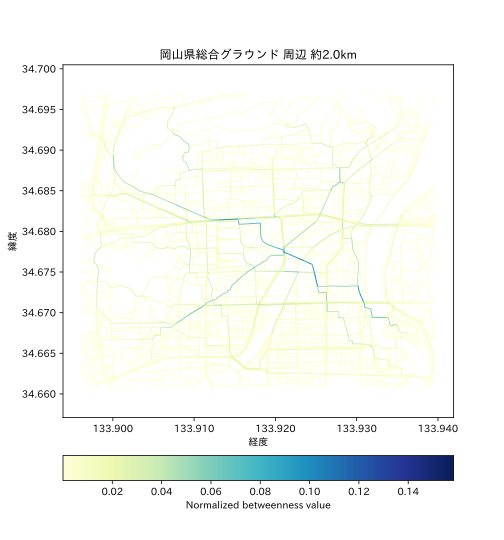
\includegraphics[width=.6\textwidth]{road-oka-with-betweenness.eps}
  \caption{実験で用いる道路ネットワーク}
  \label{fig:road-okayama}
\end{figure}

図\textcolor{red}{TODO}は辺操作後の媒介中心性の最大値の分布を表す.
辺の追加によって,最大$0.1607$の正規化された媒介中心性を
\textcolor{red}{xxx}まで減少させることに成功した.
また,辺の追加によって,最大$0.1607$の正規化された媒介中心性を
\textcolor{red}{xxx}まで減少させることに成功した.

\textcolor{red}{TODO: insert histogram of diff of min, mean, and max}

\textcolor{red}{TODO: insert figure of road indicates minimized maximum bc}

\section{媒介中心性のリアルタイム計算}

第\ref{chap:introduction}章で説明したように,社会ネットワーク分析に
おいて,媒介中心性をはじめとした中心性に注目することは重要である.
しかし,現実の社会ネットワークでは,友人関係が時間とともに出現と消滅を繰り返している.
この実験では,友人関係の出現と消滅が頻繁に起こりうる状況で,
媒介中心性をリアルタイムで計算する用途への応用を想定する.

この実験では,SFHH\cite{Genois2018}というデータセットを用いた.
このデータセットは,ある会議の参加者に赤外線タグを持たせることによって,
参加者同士の交流の様子を記録したものである.

図\ref{fig:exp-sfhh}は,そのSFHHデータセットをもとに,辺の挿入と削除を
繰り返したときの,各手法の実行時間を表す.それとともに,20秒間の
うちに発生した,挿入と削除操作の内訳を示す.

\begin{figure}[tb]
  \centering
  \includegraphics{exp-sfhh.eps}
  \caption{SFHHに対する実験結果}
  \label{fig:exp-sfhh}
\end{figure}

図より,小規模な場合ではあるが,媒介中心性をリアルタイムに計算できる.
しかし,更新の量が多い場合,Brandesのアルゴリズムの方が高速に計算していることが分かる.
今後は,多くの辺の操作に対応するアルゴリズムの開発が求められる.

\chapter{結論}
\label{chap:conclusion}
本研究は,RamalingamとRepsの最短経路更新アルゴリズムに基づく辺削除時の媒介中心性更新法の提案と評価を目的とした.
本研究で提案したアルゴリズムは,まず操作の影響を受ける分だけ媒介中心性の値を減算し,次にRamalingamとRepsに基づく方法で最短経路を更新した後,操作の影響を受けた分だけ媒介中心性の値を加算するものである.

提案法の評価は理論解析と実験によって行われた.
理論解析では,提案したアルゴリズムの時間計算量を導出し評価した.
具体的には,提案アルゴリズムを媒介中心性増減アルゴリズムと最短経路更新アルゴリズムの二つに分け,
それぞれのアルゴリズムの時間計算量を導出し,
既存法であるBrandesのアルゴリズムとDijkstraのアルゴリズムとそれぞれ比較した.
その結果,両アルゴリズムの時間計算量は各アルゴリズムによって走査される頂点の数が少ないとき,
既存アルゴリズムの時間計算量よりも小さいことを示した.

さらに実験では,提案アルゴリズムとBrandesのアルゴリズムの性能を比較した.
比較の結果,人工ネットワークと実ネットワーク両方で提案アルゴリズムの方がBrandesのアルゴリズムよりも媒介中心性の値を高速に更新することを示した.
特に,実ネットワークにおける性能比較の結果から,提案アルゴリズムはBrandesのアルゴリズムと比べて$6.87$倍の性能をもつことを示した.
さらに,提案アルゴリズムを応用して,媒介中心性の最大値を最小および最大にする辺操作の探索を行った.

今後の目標は,提案アルゴリズムを複数の辺操作に対応できるように拡張することと,
媒介中心性の最大値が最小であるようなグラフを遺伝アルゴリズムを基に探索するアルゴリズムの開発である.
%しろよ,絶対しろよ(熱い湯船の縁に掴まりながら)


\acknowledgment
本論文は筆者が岡山大学工学部情報系学科に在籍中の研究結果をまとめたものである.
本研究を行うにあたり,ご指導を頂いた岡山大学大学院自然科学研究科
産業創成工学専攻○○○○教授に深謝の意を表する.また,○○研究室の皆様には,
日常の議論を通して多くの知識や示唆を頂いた.ここに謝意を表する.

\appendix

\printbibliography[title=参考文献]

\end{document}
